\documentclass[12pt, letterpaper]{article}

% --- PAQUETES DE IDIOMA Y FORMATO ---
\usepackage[utf8]{inputenc}
\usepackage[spanish]{babel}
\usepackage[margin=2.5cm]{geometry}
\usepackage{graphicx} 
\usepackage{hyperref} 
\usepackage{xcolor}   
\usepackage{listings}
\usepackage{booktabs} 
\usepackage{float}

% --- CONFIGURACIÓN PARA EL CÓDIGO JAVA Y TEXTO PLANO ---
\definecolor{codegreen}{rgb}{0,0.6,0}
\definecolor{codegray}{rgb}{0.5,0.5,0.5}
\definecolor{codepurple}{rgb}{0.58,0,0.82}
\definecolor{backcolour}{rgb}{0.95,0.95,0.92}

\lstdefinestyle{mystyle}{
	backgroundcolor=\color{backcolour},   
	commentstyle=\color{codegreen},
	keywordstyle=\color{magenta},
	numberstyle=\tiny\color{codegray},
	stringstyle=\color{codepurple},
	basicstyle=\ttfamily\footnotesize,
	breakatwhitespace=false,         
	breaklines=true,                 
	captionpos=b,                    
	keepspaces=true,                 
	numbers=left,             
	numbersep=5pt,                  
	showspaces=false,                
	showstringspaces=false,
	showtabs=false,                  
	tabsize=2
}
\lstset{style=mystyle}

% --- INICIO DEL DOCUMENTO ---
\begin{document}
	
	% --- PORTADA ---
	\begin{titlepage}
		\centering
		\vspace*{0.5cm}
		
		
\includegraphics[width=2.8cm]{logo_unam.png} 
		\hfill
		
\includegraphics[width=2.8cm]{logo_fi.png} 
		\\[1cm] 
		
		{\Huge \textbf{Universidad Nacional Autónoma de México}}\\[0.5cm]
		{\LARGE \textbf{Facultad de Ingeniería}}\\[1cm]
		
		{\Large Asignatura: Programación Orientada a Objetos}\\[0.5cm]
		{\Large Proyecto: Sistema de Gestión y Reservación de Vuelos en Java}\\[1cm]
		
		% Título del Reporte
		\rule{\linewidth}{0.5mm} \\[0.4cm]
		{ \huge \bfseries Reporte Técnico Final: \\ Análisis, Diseño e Implementación del Sistema ``Aeroviajes'' }\\[0.4cm]
		\rule{\linewidth}{0.5mm} \\[1.5cm] 
		
		\begin{flushleft}
			\Large \textbf{Equipo de Desarrollo:}\\
			\vspace{0.3cm}
			\normalsize
			$\bullet$ Francisco José Coutiño Morales (Núm. Cta: 425121623)\\ 
			$\bullet$ Ernesto Flamenco Villaseñor (Núm. Cta: 319170599)\\
		\end{flushleft}
		
		\vfill 
		
		{\large 29 de mayo de 2026} 
	\end{titlepage}
	
	% --- ÍNDICE ---
	\newpage
	\tableofcontents
	\newpage
	
	% =========================================================================
	% --- SECCIÓN 1: INTRODUCCIÓN ---
	% =========================================================================
	\section{Introducción}
	El presente documento detalla la arquitectura, las decisiones de diseño y el flujo de desarrollo del proyecto \textbf{Aeroviajes}, un sistema de gestión y reservación de vuelos codificado íntegramente en Java sobre el IDE Apache NetBeans 21. El sistema integra los paradigmas de la Programación Orientada a Objetos (POO) \cite{oracle_oop}, el \textit{Java Collections Framework} \cite{oracle_collections}, persistencia mediante serialización de objetos, programación concurrente con hilos y la aplicación de seis patrones de diseño clásicos del catálogo GoF \cite{gof}.
	
	El objetivo fundamental del proyecto fue modelar un escenario comercial real —el de una aerolínea que debe gestionar usuarios, vuelos, reservas y boletos— y construir un sistema funcional completo con interfaz gráfica de usuario en Java Swing, control de acceso por roles (administrador y cliente) y persistencia transaccional. A diferencia de un sistema de consola, Aeroviajes implementa una arquitectura por capas que separa claramente la presentación, la lógica de negocio, la persistencia y el dominio, demostrando así un nivel de madurez arquitectónica apto tanto para evaluación académica como para servir como pieza de portafolio profesional.
	
	% =========================================================================
	% --- SECCIÓN 2: OBJETIVOS DEL PROYECTO ---
	% =========================================================================
	\section{Objetivos del Proyecto}
	\textbf{Objetivo general:} Desarrollar un sistema de reservación de vuelos en Java aplicando todos los conceptos del curso de Programación Orientada a Objetos, integrando además patrones de diseño, concurrencia y una interfaz gráfica funcional.
	
	\textbf{Objetivos específicos:}
	\begin{itemize}
		\item Diseñar una arquitectura por capas con separación estricta de responsabilidades.
		\item Implementar un esquema de control de acceso diferenciado entre administradores y clientes, validado en tiempo de ejecución.
		\item Aplicar los seis patrones de diseño GoF que cubran las tres categorías clásicas (creacionales, estructurales y conductuales).
		\item Integrar programación concurrente mediante hilos y estructuras \textit{thread-safe}, acopladas a la lógica de negocio mediante el patrón Productor-Consumidor.
		\item Persistir todos los datos del sistema (usuarios, vuelos, reservas) mediante serialización de objetos para garantizar continuidad entre ejecuciones.
		\item Producir una interfaz gráfica navegable, intuitiva y profesional.
	\end{itemize}
	
	% =========================================================================
	% --- SECCIÓN 3: FLUJO DE TRABAJO ---
	% =========================================================================
	\section{Flujo de Trabajo y Metodología de Desarrollo}
	El desarrollo siguió un enfoque iterativo e incremental, con repartición vertical del trabajo entre los dos integrantes del equipo. La metodología se dividió en cuatro fases principales:
	
	\begin{enumerate}
		\item \textbf{Fase de diseño conceptual:} Se definieron las entidades del dominio, los paquetes lógicos y los patrones de diseño aplicables. Se elaboró un diagrama UML preliminar con PlantUML, un README profesional para el repositorio GitHub y un cronograma de trabajo dividido por días y por responsable. El repositorio se configuró como repositorio público en GitHub con el nombre \texttt{Sitema-de-Gestion-y-Reservacion-de-Vuelos}, bajo licencia MIT.
		
		\item \textbf{Fase de codificación en paralelo:} El equipo dividió la responsabilidad por capas verticales para minimizar las dependencias cruzadas. Francisco se encargó del paquete \texttt{model} (entidades del dominio), \texttt{persistence} (repositorios y manejo de archivos), los patrones Singleton, Factory y Flyweight, el paquete \texttt{util} y la GUI de autenticación y administración. Ernesto se encargó del paquete \texttt{exception}, el paquete \texttt{service} (gestores de negocio), los patrones Strategy, Observer y Proxy, el paquete \texttt{threads} y la GUI del flujo cliente. Esta división permitió que ambos avanzaran sin bloquearse mutuamente, ya que las únicas dependencias críticas eran \texttt{model} y \texttt{exception}, que se construyeron primero.
		
		\item \textbf{Fase de integración:} Una vez que ambos integrantes subieron sus paquetes al repositorio compartido, se procedió a integrar las piezas. Durante esta fase se detectaron incompatibilidades entre las firmas de métodos esperadas por cada lado (descritas en la Sección 7), las cuales se resolvieron mediante ajustes en las clases del modelo y los gestores, sin requerir reescrituras profundas. La \texttt{VentanaPrincipal} fue refactorizada para instanciar y coordinar todos los servicios, repositorios e hilos del sistema.
		
		\item \textbf{Fase de pruebas funcionales y documentación:} Se ejecutó un \textit{smoke test} manual del flujo completo (registro $\rightarrow$ login $\rightarrow$ consulta $\rightarrow$ compra $\rightarrow$ ticket $\rightarrow$ cierre $\rightarrow$ reinicio $\rightarrow$ verificación de persistencia) para validar que todas las capas funcionaran end-to-end. Se redactaron el reporte técnico, el manual de usuario y se actualizó el diagrama UML al estado \textit{As-Built}.
	\end{enumerate}
	
	% =========================================================================
	% --- SECCIÓN 4: ARQUITECTURA DEL SISTEMA ---
	% =========================================================================
	\section{Arquitectura del Sistema}
	El sistema sigue una \textbf{arquitectura por capas} con dependencias unidireccionales descendentes:
	
	\begin{lstlisting}[basicstyle=\ttfamily\footnotesize, backgroundcolor=\color{backcolour}, numbers=none]
		+------------------------------------------------------+
		| Capa de Presentacion   . aeroviajes.ui               | <- Swing (JFrame, JPanel)
		+------------------------------------------------------+
		| Capa de Servicio       . aeroviajes.service          | <- Logica de negocio
		+------------------------------------------------------+
		| Capa de Persistencia   . aeroviajes.persistence      | <- Archivos / serializacion
		+------------------------------------------------------+
		| Capa de Dominio        . aeroviajes.model            | <- Entidades del negocio
		+------------------------------------------------------+
		^ patterns . threads . exception . util (transversales)
	\end{lstlisting}
	
	La presentación depende del servicio, el servicio del dominio y de la persistencia, pero \textbf{nunca al revés}. Las capas transversales (patrones, hilos, excepciones, utilidades) son consumidas por todas las anteriores sin acoplarlas entre sí. Esta separación facilita el mantenimiento, las pruebas y la extensibilidad del sistema.
	
	% =========================================================================
	% --- SECCIÓN 5: ANÁLISIS DE CONCEPTOS POO ---
	% =========================================================================
	\section{Análisis de los Conceptos POO Implementados}
	A continuación se detalla cómo se aplicó cada uno de los conceptos requeridos por la rúbrica, indicando ubicación específica en el código y la justificación de diseño detrás de cada decisión.
	
	\subsection{Uso de Paquetes y Estructura Modular}
	El proyecto está organizado en \textbf{ocho paquetes lógicos} que reflejan la arquitectura por capas. Esta separación no es decorativa: cada paquete encapsula una responsabilidad única y oculta sus detalles internos del resto del sistema. La estructura es la siguiente:
	
	\begin{table}[H]
		\centering
		\renewcommand{\arraystretch}{1.2}
		\begin{tabular}{p{4.5cm} p{10cm}}
			\toprule
			\textbf{Paquete} & \textbf{Responsabilidad} \\
			\midrule
			\texttt{aeroviajes.model} & Entidades del dominio del negocio (Usuario, Vuelo, Reserva, Ticket, Aeropuerto, Aerolínea). \\
			\texttt{aeroviajes.service} & Lógica de negocio (gestores de usuarios, vuelos, reservas y tickets). \\
			\texttt{aeroviajes.persistence} & Repositorios y manejo de archivos (serialización a \texttt{.dat} y escritura de tickets \texttt{.txt}). \\
			\texttt{aeroviajes.exception} & Excepciones personalizadas del dominio. \\
			\texttt{aeroviajes.patterns} & Implementaciones de los seis patrones GoF, divididas en seis sub-paquetes. \\
			\texttt{aeroviajes.threads} & Hilos y la cola \textit{thread-safe} del patrón Productor-Consumidor. \\
			\texttt{aeroviajes.ui} & Interfaz gráfica de usuario (JFrame y paneles Swing). \\
			\texttt{aeroviajes.util} & Utilidades transversales (generadores, validadores, constantes). \\
			\bottomrule
		\end{tabular}
	\end{table}
	
	El paquete \texttt{patterns} se subdivide internamente en \texttt{singleton}, \texttt{factory}, \texttt{flyweight}, \texttt{proxy}, \texttt{strategy} y \texttt{observer}, agrupando cada patrón en su propia carpeta. Esta organización facilita identificar dónde vive cada patrón y explicarlo en una exposición.
	
	\subsection{Modificadores de Acceso}
	El sistema aplica los cuatro niveles de acceso de Java de forma consciente y consistente, encapsulando el estado interno de las entidades y exponiendo únicamente las operaciones necesarias.
	
	\begin{itemize}
		\item \textbf{\texttt{private}:} atributos de todas las entidades del modelo. La contraseña del \texttt{Usuario} es un ejemplo crítico: se almacena como \texttt{private} y \textbf{no se expone mediante getter}, forzando al resto del sistema a usar el método \texttt{validarContrasena(String intento)} para verificarla. Esto previene fugas accidentales de credenciales.
		\item \textbf{\texttt{protected}:} usado en la clase abstracta \texttt{Usuario} para que sus subclases (\texttt{Administrador} y \texttt{Cliente}) puedan acceder a los atributos heredados sin exponerlos al exterior. Su constructor es también \texttt{protected} para impedir instanciación directa.
		\item \textbf{\texttt{public}:} reservado para la API que cada clase ofrece al sistema (constructores, métodos de negocio, getters).
		\item \textbf{Package-private (sin modificador):} utilizado en clases internas de implementación que no deben ser visibles fuera de su paquete.
	\end{itemize}
	
	Adicionalmente, los atributos inmutables (como el \texttt{id} de un \texttt{Vuelo}, los códigos IATA de un \texttt{Aeropuerto} o el \texttt{codigoTicket}) se declaran como \texttt{private final}, garantizando que no pueden alterarse tras la construcción del objeto. Las clases que implementan el patrón Flyweight (\texttt{Aeropuerto}, \texttt{Aerolinea}) están declaradas como \texttt{public final}, impidiendo su extensión y reforzando su inmutabilidad.
	
	\subsection{Herencia y Polimorfismo}
	El sistema demuestra herencia y polimorfismo en cinco jerarquías distintas, todas con propósito funcional real:
	
	\begin{enumerate}
		\item \textbf{Jerarquía de usuarios:} La clase abstracta \texttt{Usuario} define los atributos comunes y el método abstracto \texttt{getRol()}. Sus dos subclases concretas, \texttt{Administrador} y \texttt{Cliente}, sobrescriben este método. Adicionalmente, \texttt{Cliente} agrega un historial de reservas mediante una colección \texttt{List<Reserva>}. Esto habilita el flujo polimórfico en el login: tras autenticar al usuario, el sistema invoca \texttt{u.getRol()} sin conocer la subclase concreta.
		\item \textbf{Implementaciones de \texttt{IRepositorio<T>}:} Tres clases (\texttt{RepositorioUsuarios}, \texttt{RepositorioVuelos}, \texttt{RepositorioReservas}) heredan de la clase abstracta genérica \texttt{RepositorioBase<T>}. Cada subclase reutiliza toda la lógica CRUD definida en la base (principio DRY).
		\item \textbf{Implementaciones de \texttt{IGestorVuelos}:} Dos clases (\texttt{GestorVuelosReal} y \texttt{GestorVuelosProxy}) implementan la misma interfaz. El proxy envuelve al real e intercepta las operaciones de modificación para validar permisos.
		\item \textbf{Implementaciones de \texttt{IValidadorPago}:} \texttt{ValidadorTarjetaCredito} y \texttt{ValidadorTarjetaDebito} implementan la misma interfaz, intercambiables en tiempo de ejecución (patrón Strategy).
		\item \textbf{Jerarquía de hilos:} \texttt{HiloConsumidorTickets} extiende \texttt{Thread}, \texttt{HiloAutoGuardado} implementa \texttt{Runnable} y \texttt{HiloCargaVuelos} extiende \texttt{SwingWorker}. Cada uno demuestra una forma distinta de heredar el comportamiento concurrente de Java.
	\end{enumerate}
	
	\subsection{Clases Abstractas e Interfaces}
	El sistema implementa dos clases abstractas y cinco interfaces:
	
	\textbf{Clases abstractas:}
	\begin{itemize}
		\item \texttt{Usuario} (en \texttt{model}): define la estructura común pero no puede instanciarse directamente. Obliga a implementar \texttt{getRol()}.
		\item \texttt{RepositorioBase<T>} (en \texttt{persistence}): centraliza la lógica CRUD genérica y define el método abstracto \texttt{obtenerId(T entidad)}. Este es el patrón \textbf{Template Method}.
	\end{itemize}
	
	\textbf{Interfaces:}
	\begin{itemize}
		\item \texttt{IRepositorio<T>}: contrato genérico de los repositorios.
		\item \texttt{IGestorVuelos}: contrato del gestor de vuelos.
		\item \texttt{IValidadorPago}: contrato de los validadores de pago.
		\item \texttt{IObservadorReserva}: contrato de los observadores para notificaciones.
		\item \texttt{PanelActualizable}: permite callbacks \texttt{alMostrarse()} en paneles Swing.
	\end{itemize}
	
	\subsection{Colecciones}
	El proyecto utiliza intensivamente el Java Collections Framework:
	
	\begin{itemize}
		\item \textbf{\texttt{ArrayList<T>}:} en \texttt{RepositorioBase} para mantener la colección de entidades en memoria. Elegido por su acceso secuencial eficiente.
		\item \textbf{\texttt{HashMap<String, Usuario>}:} en \texttt{GestorUsuarios} para indexar los usuarios por su correo electrónico en tiempo constante O(1) \cite{oracle_hashmap}.
		\item \textbf{\texttt{HashMap<String, Vuelo>}:} en \texttt{GestorVuelosReal} por la misma razón.
		\item \textbf{\texttt{HashMap<String, Aeropuerto>}} y \textbf{\texttt{HashMap<String, Aerolinea>}:} en las fábricas Flyweight, cachean las instancias.
		\item \textbf{\texttt{BlockingQueue<Reserva>}:} cola \textit{thread-safe} que sirve de puente entre el hilo de la GUI y el hilo trabajador del patrón Productor-Consumidor \cite{oracle_blockingqueue}.
		\item \textbf{\texttt{List<T>} como tipo de retorno:} los repositorios devuelven copias defensivas de la interfaz para impedir que el llamador modifique la colección interna.
	\end{itemize}
	
	\subsection{Manejo de Excepciones}
	El sistema define \textbf{seis excepciones personalizadas} que heredan de \texttt{Exception} (verificadas):
	
	\begin{table}[H]
		\centering
		\renewcommand{\arraystretch}{1.2}
		\begin{tabular}{p{4.5cm} p{10cm}}
			\toprule
			\textbf{Excepción} & \textbf{Cuándo se lanza} \\
			\midrule
			\texttt{VueloNoDisponible} & Al intentar acceder a un vuelo cuyo id no existe. \\
			\texttt{AsientoNoDisponible} & Al intentar reservar un asiento en un vuelo lleno. \\
			\texttt{UsuarioNoEncontrado} & Al buscar un usuario que no existe en el sistema. \\
			\texttt{UsuarioYaExiste} & Al intentar registrar un correo ya tomado. \\
			\texttt{Autenticacion} & Cuando una operación está protegida o una contraseña es incorrecta. \\
			\texttt{PagoInvalido} & Cuando la validación de un método de pago falla. \\
			\bottomrule
		\end{tabular}
	\end{table}
	
	\subsection{Manejo de Archivos}
	La persistencia se basa en la \textbf{serialización nativa de Java} (\texttt{Serializable}). La capa está estructurada en dos niveles:
	\begin{itemize}
		\item \textbf{Nivel bajo (\texttt{GestorArchivos}):} Clase de utilidad estática que encapsula \texttt{ObjectOutputStream} y \texttt{ObjectInputStream}.
		\item \textbf{Nivel alto (Repositorios):} \texttt{cargar()} se invoca automáticamente en el constructor, y \texttt{persistir()} se llama tras cada operación de modificación.
	\end{itemize}
	
	\subsection{Patrones de Diseño}
	El sistema implementa \textbf{seis patrones GoF} \cite{gof}:
	
	\begin{itemize}
		\item \textbf{Singleton (\texttt{SistemaAeroviajes}):} garantiza una única instancia coordinadora.
		\item \textbf{Factory Method (\texttt{UsuarioFactory}):} centraliza la creación de subtipos de \texttt{Usuario}.
		\item \textbf{Flyweight (\texttt{AeropuertoFlyweightFactory}):} optimiza memoria compartiendo las instancias de aeropuertos y aerolíneas.
		\item \textbf{Proxy (\texttt{GestorVuelosProxy}):} aplica un \textit{Protection Proxy} para validar permisos de administrador.
		\item \textbf{Strategy (\texttt{IValidadorPago}):} encapsula algoritmos de validación en clases intercambiables.
		\item \textbf{Observer (\texttt{NotificadorReservas}):} notifica eventos a los observadores suscritos desacoplando la lógica.
		\item \textbf{Patrón de concurrencia: Productor-Consumidor.}
	\end{itemize}
	
	% =========================================================================
	% --- SECCIÓN 6: DESARROLLO DEL PROYECTO ---
	% =========================================================================
	\section{Desarrollo del Proyecto}
	La implementación del sistema se construyó capa por capa, de abajo hacia arriba:
	
	\textbf{Capa de dominio.} Se comenzó por el paquete \texttt{model}, definiendo las ocho entidades centrales.
	
	\textbf{Capa de persistencia.} Se diseñó la interfaz \texttt{IRepositorio<T>} y la clase \texttt{RepositorioBase<T>}.
	
	\textbf{Capa de excepciones.} Se definieron las excepciones verificadas.
	
	\textbf{Capa de servicio.} Se construyeron los cuatro gestores (\texttt{GestorUsuarios}, \texttt{GestorVuelosReal}, \texttt{GestorReservas}, \texttt{GestorTickets}).
	
	\textbf{Capa de patrones.} Se desarrollaron los seis sub-paquetes arquitectónicos.
	
	\textbf{Capa de hilos.} Implementación de \texttt{ColaTickets} y los tres procesos en segundo plano.
	
	\textbf{Capa de presentación.} Interfaz en Swing con un único \texttt{JFrame} y patrón \texttt{CardLayout}.
	
	% =========================================================================
	% --- SECCIÓN 7: ERRORES DE INTEGRACIÓN ---
	% =========================================================================
	\section{Detección y Corrección de Errores de Integración}
	Al fusionar los paquetes desarrollados en paralelo, surgieron incompatibilidades que fueron corregidas:
	
	\begin{enumerate}
		\item \textbf{Discrepancia en constructores:} Se ajustaron las llamadas en \texttt{GestorUsuarios} para generar el ID automáticamente mediante \texttt{UUID}.
		\item \textbf{Acceso a la contraseña:} Se refactorizó el gestor para usar \texttt{u.validarContrasena(input)} respetando el encapsulamiento.
		\item \textbf{Nombres de getters:} Se homogeneizaron las llamadas desde la UI al modelo.
		\item \textbf{Falta de persistencia en \texttt{GestorVuelosReal}:} Se solucionó cargando y guardando desde \texttt{RepositorioVuelos} en cada mutación.
		\item \textbf{Refactorización de \texttt{PanelLogin}:} Se simplificó la navegación al panel de administrador una vez que este fue desarrollado.
	\end{enumerate}
	
	% =========================================================================
	% --- SECCIÓN 8: DIAGRAMA DE CLASES ---
	% =========================================================================
	\section{Diagrama de Clases Final (As-Built)}
	A continuación se muestra el diagrama UML de clases con la arquitectura definitiva del sistema, incluyendo todos los paquetes, las relaciones de herencia, implementación de interfaces, composición y dependencia.
	
	\begin{figure}[H]
		\centering
		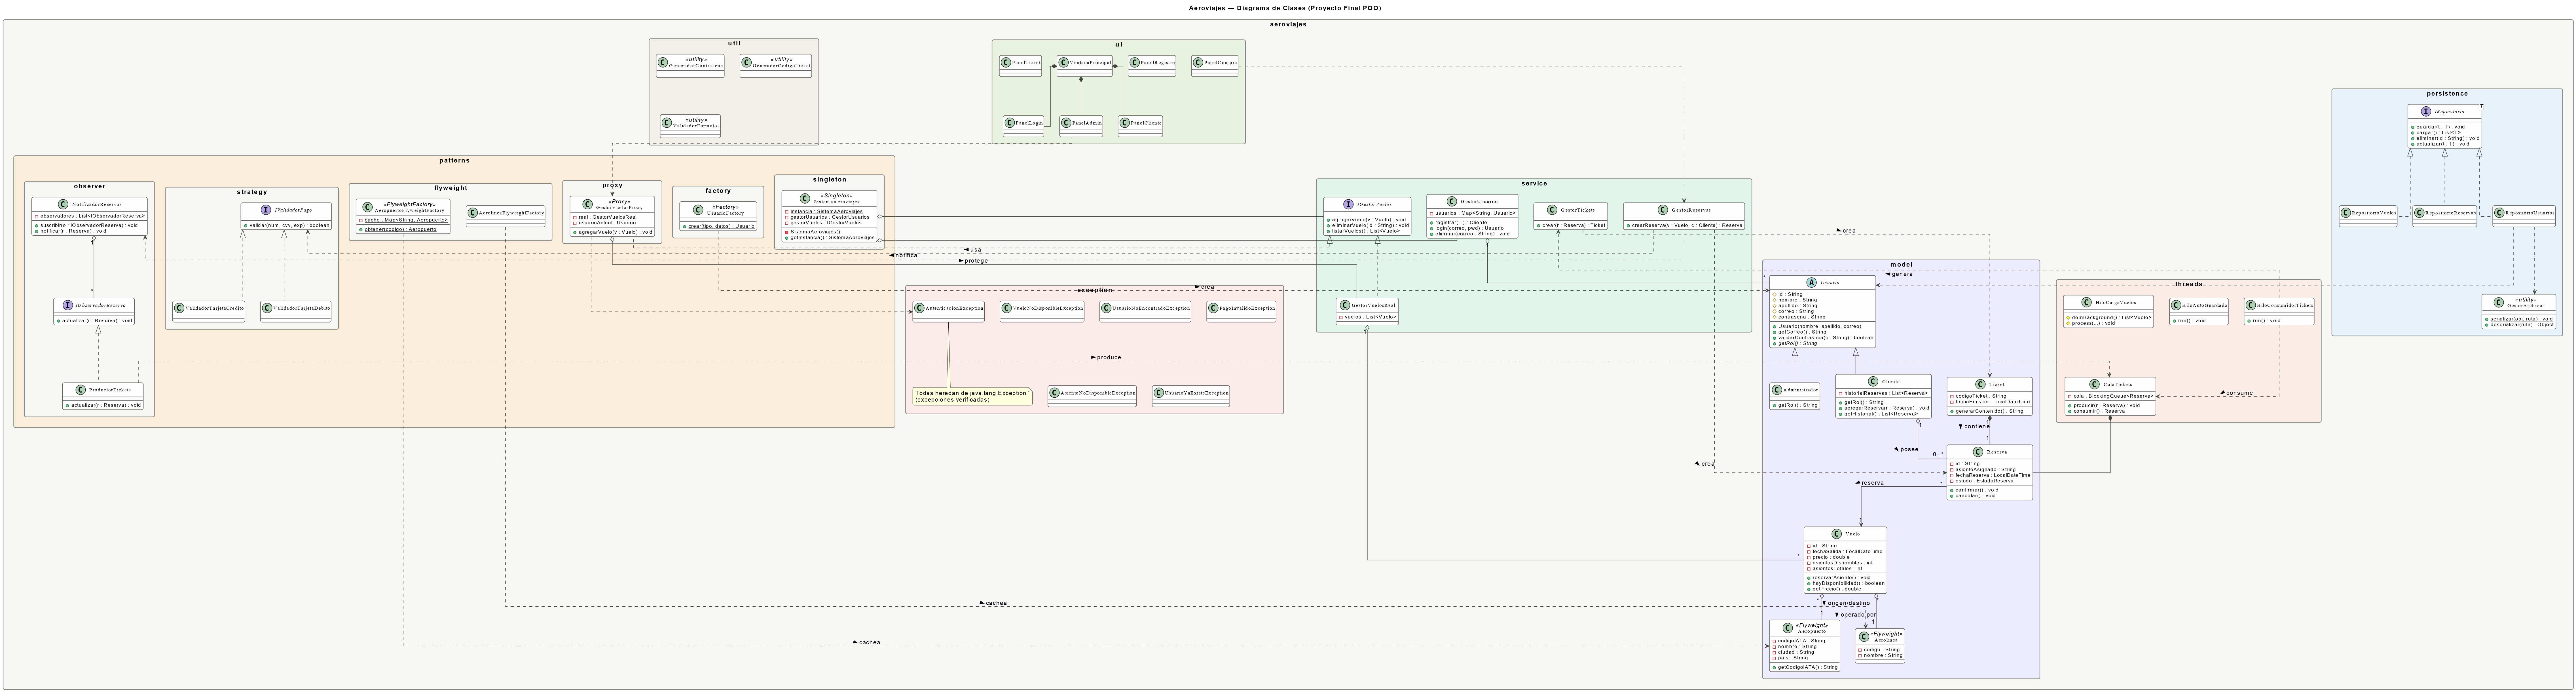
\includegraphics[width=\textwidth]{Sistema de Gestion y Reservacion de Vuelos - Diagrama de Clases_page-0001.jpg}
		\caption{Diagrama de clases final (As-Built) del sistema Aeroviajes.}
		\label{fig:diagrama_final}
	\end{figure}
	
	El diagrama agrupa visualmente los ocho paquetes mediante colores distintos: \texttt{util} y \texttt{ui} (presentación y soporte), \texttt{patterns} con sus seis sub-paquetes (singleton, strategy, flyweight, proxy, factory, observer), \texttt{service} (lógica de negocio), \texttt{exception} (excepciones del dominio), \texttt{model} (entidades), \texttt{persistence} (repositorios) y \texttt{threads} (hilos). Las relaciones tipadas muestran cómo se conectan: herencia para la jerarquía \texttt{Usuario} $\rightarrow$ \texttt{Administrador}/\texttt{Cliente}, implementación de interfaces para los repositorios y validadores, agregación entre \texttt{Cliente} y sus reservas, y composición fuerte entre \texttt{Ticket} y \texttt{Reserva}. Las flechas con estereotipos (\texttt{«crea»}, \texttt{«notifica»}, \texttt{«protege»}, \texttt{«cachea»}, \texttt{«produce»}, \texttt{«consume»}) expresan la dirección y el rol de cada dependencia, comunicando la dinámica del sistema más allá de la pura estructura.
	
	% =========================================================================
	% --- SECCIÓN 9: CONCLUSIONES ---
	% =========================================================================
	\section{Conclusiones Individuales}
	
	\subsection{Francisco José Coutiño Morales}
	El desarrollo de Aeroviajes representó para mí un salto  respecto a los proyectos y practicas anteriores del curso. Diseñamos desde el inicio una arquitectura por capas con ocho paquetes lógicos, interfaz gráfica completa, persistencia transaccional y seis patrones de diseño cuidadosamente seleccionados. 
	
	Lo más difisil pero importante del proceso fue entender que \textbf{los patrones de diseño que expusimos en la clase y el como implementarlos en el proyecto, abarcando todos los temas posibles del curso}, y como estos son respuestas concretas a problemas reales: el Flyweight, por ejemplo, no se justifica "porque está en GoF", se justifica porque cien vuelos comparten diez aeropuertos y duplicar esos datos sería un desperdicio de memoria.
	
	La aplicación del Template Method en \texttt{RepositorioBase<T>} fue uno de los momentos más satisfactorios del proyecto: ver cómo trescientas líneas de lógica CRUD se centralizan en una clase abstracta y los repositorios concretos quedan reducidos a quince líneas cada uno es la mejor demostración del principio DRY que se puede pedir. El proyecto también puso a prueba habilidades que no son estrictamente técnicas: coordinación con Ernesto sobre firmas de métodos antes de programar en paralelo y la resolución de problemas bajo presión de tiempo, que fue lo que mas nos costo y por lo que nos sirvio mucho los dias extra que nos dio para la entrega del proyecto.
	
	\subsection{Ernesto Flamenco Villaseñor}
	Trabajar en el Sistema de Gestion y Reservacion de Vuelos - Aeroviajes me permitió consolidar conceptos que en cursos anteriores había aplicado de forma aislada. La parte que más disfruté fue diseñar el flujo del patrón Productor-Consumidor acoplado al Observer: cuando vi por primera vez en la consola el mensaje "Reserva en cola" seguido del consumidor procesándola en un hilo separado, entendí en concreto qué significa la concurrencia útil.
	
	Implementar el Proxy fue particularmente revelador: la elegancia de poder interceptar cada operación crítica y validar el rol del usuario sin tocar la implementación real demostró el concepto y alcance que tiene el polimorfismo. El trabajo en equipo tuvo sus retos, pero me enseñó que la coordinación previa es una necesidad cuando dos personas trabajan en paralelo. Considero que cumplimos con los objetivos planteados al inicio del proyecto.
	
	% =========================================================================
	% --- BIBLIOGRAFÍA ---
	% =========================================================================
	\newpage
	\renewcommand{\refname}{Bibliografía}
	\begin{thebibliography}{9}
		
		\bibitem{oracle_oop} 
		Oracle. (s.f.). \textit{Lesson: Object-Oriented Programming Concepts}. The Java Tutorials. Recuperado de \url{https://docs.oracle.com/javase/tutorial/java/concepts/index.html}
		
		\bibitem{oracle_collections} 
		Oracle. (s.f.). \textit{Lesson: Introduction to Collections}. The Java Tutorials. Recuperado de \url{https://docs.oracle.com/javase/tutorial/collections/intro/index.html}
		
		\bibitem{gof} 
		Gamma, E., Helm, R., Johnson, R., \& Vlissides, J. (1994). \textit{Design Patterns: Elements of Reusable Object-Oriented Software}. Addison-Wesley.
		
		\bibitem{java_concurrency} 
		Goetz, B., Peierls, T., Bloch, J., Bowbeer, J., Holmes, D., \& Lea, D. (2006). \textit{Java Concurrency in Practice}. Addison-Wesley.
		
		\bibitem{oracle_hashmap} 
		Oracle. (s.f.). \textit{Class HashMap<K,V>}. Java Platform, Standard Edition 21 API Specification. Recuperado de \url{https://docs.oracle.com/en/java/javase/21/docs/api/java.base/java/util/HashMap.html}
		
		\bibitem{oracle_blockingqueue} 
		Oracle. (s.f.). \textit{Interface BlockingQueue<E>}. Java Platform, Standard Edition 21 API Specification. Recuperado de \url{https://docs.oracle.com/en/java/javase/21/docs/api/java.base/java/util/concurrent/BlockingQueue.html}
		
		\bibitem{bell_parr_java}
		Bell, D., \& Parr, M. (2003). \textit{Java para estudiantes} (3\textsuperscript{a} ed.). Pearson Educación.
		
	\end{thebibliography}
	
\end{document}